\section{Introduction}
\label{sec:intro}

Planning with a learned model is a conceptually simple framework for reinforcement learning and data-driven decision-making.
Its appeal comes from employing learning techniques only where they are the most mature and effective: for the approximation of unknown environment dynamics in what amounts to a supervised learning problem.
Afterwards, the learned model may be plugged into classical trajectory optimization routines \cite{tassa2012synthesis,posa2014direct,matthew2017trajectory},
which are similarly well-understood in their original context.
\vspace{1em}

\begin{figure}
\centering
\begin{tikzpicture}
    \node[anchor=south west,inner sep=0] (image) at (0,0)
        {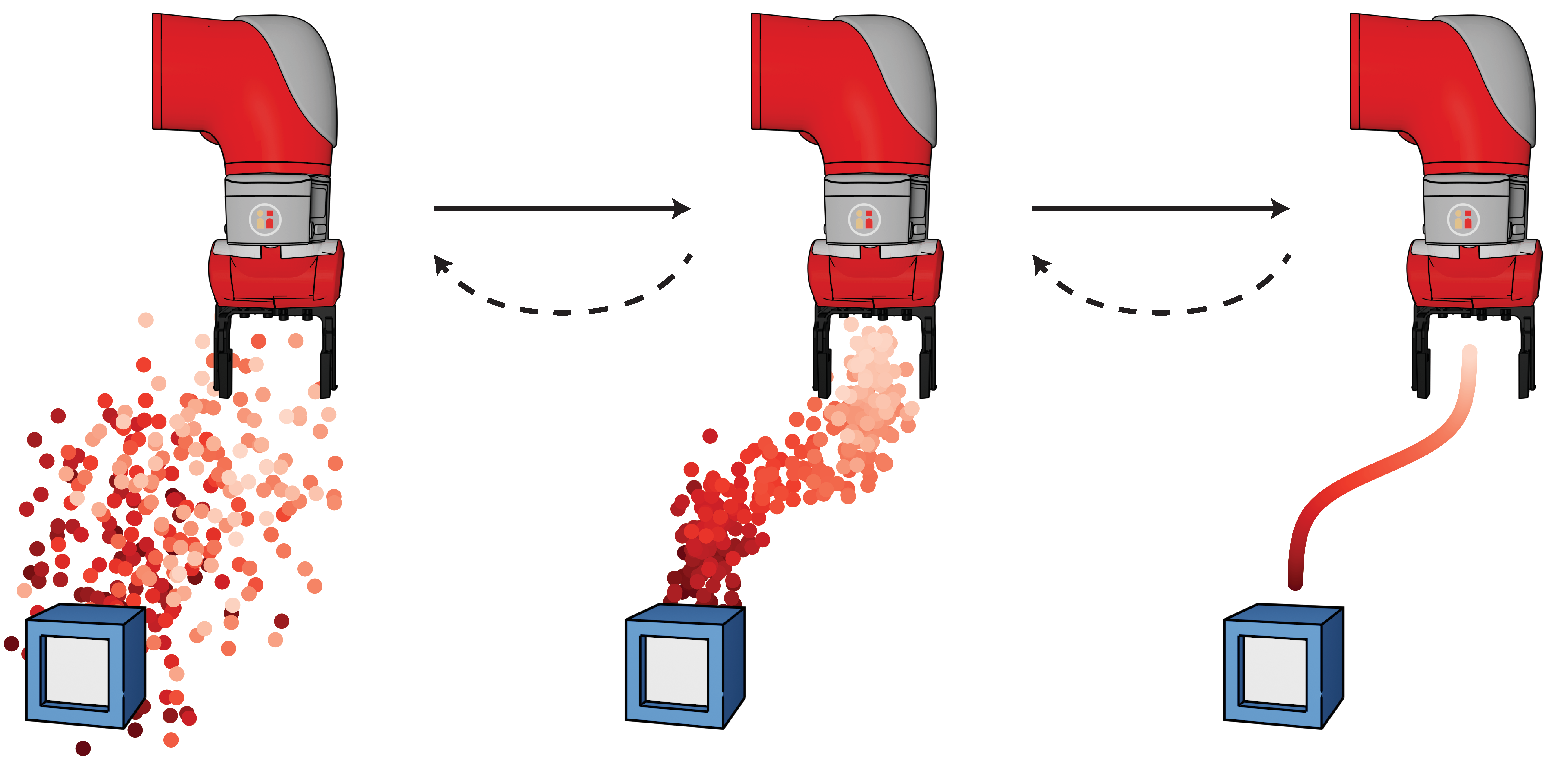
\includegraphics[width=\columnwidth]{images/teaser.pdf}};
    \begin{scope}[x={(image.south east)},y={(image.north west)}]
        \node[] at (.74,.825) {$p_\theta(\btau{i-1} \!\mid\! \btau{i})$};
        \node[] at (.74,.5) {$q(\btau{i} \!\mid\! \btau{i-1})$};
        \node[] at (.355,.825) {\small denoising};
        \node[] at (.355,.515) {\small diffusion};
    \end{scope}
\end{tikzpicture}
\vspace{-1.5em}
\caption{
    \method{} is a diffusion probabilistic model that plans by iteratively refining trajectories.
}
\vspace{-1em}
\label{fig:teaser}
\end{figure}

However, this combination rarely works as described.
Because powerful trajectory optimizers exploit learned models, plans generated by this procedure often look more like adversarial examples than optimal trajectories \cite{talvitie2014hallcuinated,ke2018modeling}.
As a result, contemporary model-based reinforcement learning algorithms often inherit more from model-free methods, such as value functions and policy gradients \cite{wang2019benchmarking}, than from the trajectory optimization toolbox.
Those methods that do rely on online planning tend to use simple gradient-free trajectory optimization routines like random shooting \cite{nagabandi2018mbmf} or the cross-entropy method \cite{botev2013cem,chua2018pets} to avoid the aforementioned issues.
\blfootnote{
\noindent Code and visualizations of the learned denoising process are available at \textbf{\href{https://diffusion-planning.github.io/}
    {\texttt{diffusion-planning.github.io}}}.
}

In this work, we propose an alternative approach to data-driven trajectory optimization.
The core idea is to train a model that is directly amenable to trajectory optimization, in the sense that sampling from the model and planning with it become nearly identical.
This goal requires a shift in how the model is designed.
Because learned dynamics models are normally meant to be proxies
for environment dynamics, improvements are often achieved by structuring the model according to the underlying causal process \cite{bapst2019structured}.
Instead, we consider how to design a model in line with the planning problem in which it will be used.
For example, because the model will ultimately be used for planning, action distributions are just as important as state dynamics and long-horizon accuracy is more important than single-step error.
On the other hand, the model should remain agnostic to reward function so that it may be used in multiple tasks, including those unseen during training.
Finally, the model should be designed so that its plans, and not just its predictions, improve with experience and are resistant to the myopic failure modes of standard shooting-based planning algorithms.

\begin{figure}
\centering
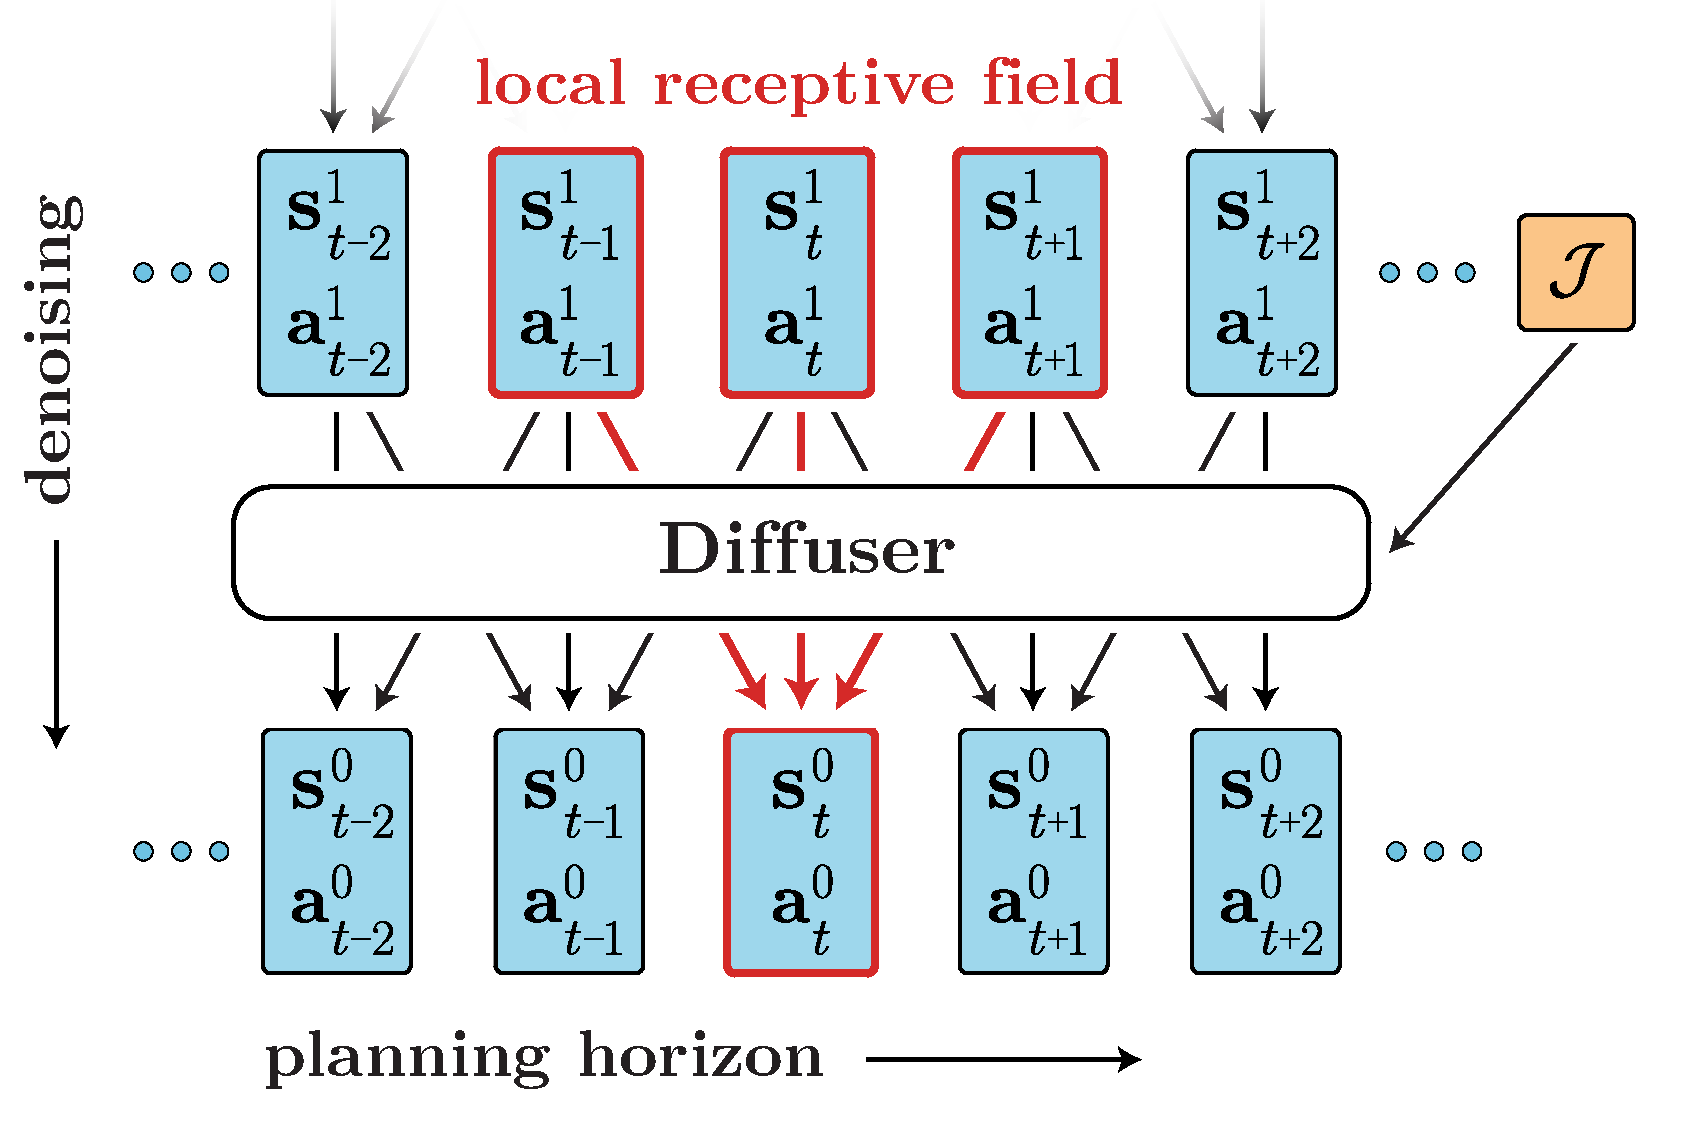
\includegraphics[width=\columnwidth]{images/diffuser_schematic.pdf}
% \vspace{-1em}
\caption{
    Diffuser samples plans by iteratively denoising two-dimensional arrays consisting of a variable number of state-action pairs.
    A small receptive field constrains the model to only enforce local consistency during a single denoising step.
    By composing many denoising steps together, local consistency can drive global coherence of a sampled plan.
    An optional guide function $\mathcal{J}$ can be used to bias plans toward those optimizing a test-time objective or satisfying a set of constraints.
}
\vspace{-1.5em}
\label{fig:architecture}
\end{figure}

We instantiate this idea as a trajectory-level diffusion probabilistic model \citep{sohldickstein2015nonequilibrium,ho2020denoising} called \method{}, visualized in Figure~\ref{fig:architecture}.
Whereas standard model-based planning techniques predict forward in time autoregressively, \method{} predicts all timesteps of a plan simultaneously.
The iterative sampling process of diffusion models leads to flexible conditioning, allowing for auxiliary guides to modify the sampling procedure to recover trajectories with high return or satisfying a set of constraints.
This formulation of data-driven trajectory optimization has several appealing properties:

\textbf{Long-horizon scalability~~}
Diffuser is trained for the accuracy of its generated trajectories rather than its single-step error, so it does not suffer from the compounding rollout errors of single-step dynamics models and scales more gracefully with respect to long planning horizon.

\textbf{Task compositionality~~}
Reward functions provide auxiliary gradients to be used while sampling a plan, allowing for a straightforward way of planning by composing multiple rewards simultaneously by adding together their gradients.

\textbf{Temporal compositionality~~}
Diffuser generates globally coherent trajectories by iteratively improving local consistency, allowing it to generalize to novel trajectories by stitching together in-distribution subsequences.

\textbf{Effective non-greedy planning~~}
By blurring the line between model and planner, the training procedure that improves the model's predictions also has the effect of improving its planning capabilities.
This design yields a learned planner that can solve the types of long-horizon, sparse-reward problems that prove difficult for many conventional planning methods.

The core contribution of this work is a denoising diffusion model designed for trajectory data and an associated probabilistic framework for behavior synthesis.
While unconventional compared to the types of models routinely used in deep model-based reinforcement learning, we demonstrate that \method has a number of useful properties and is particularly effective in offline control settings that require long-horizon reasoning and test-time flexibility.
